\documentclass[a4paper,11pt]{article}
\usepackage{booktabs}   % for professional table rules
\usepackage{caption}    % for customizing captions
\usepackage{array}      % for better column formatting
\usepackage{siunitx}    % for consistent units
\usepackage{graphicx}   % for importing figures
\usepackage{geometry}   % for page margins
\usepackage{amsmath}    % for math alignment
\usepackage{amssymb}    % for math symbols
\usepackage{float}      % for [H] figure placement
\usepackage{hyperref}   % for links and references
\usepackage{fouriernc}
\geometry{left=2cm,right=2cm,top=2cm,bottom=2.5cm}
\hypersetup{
    colorlinks=true,
    linkcolor=blue,
    filecolor=magenta,      
    urlcolor=cyan,
    pdftitle={Lab Report: Franck-Hertz Experiment},
    pdfpagemode=FullScreen,
}

\begin{document}

% ------------------- Title / Cover Page -------------------
\noindent
\begin{center}
    
\includegraphics[width=0.25\textwidth]{sut.jpg} \\
    \vspace{2pt}
\end{center}
\begin{center}
    {\LARGE \bf Department of Physics} \\
    \vspace{2pt}
    {\Large \bf Sharif University of Technology} \\
    \vspace{8pt}
    {\large \bf Physics Lab IV --- General Physics Laboratory} \\
    \vspace{4pt}
    \hrule
    \vspace{6pt}
    {\Large \bf Experiment Report: The Franck-Hertz Experiment}
\end{center}
\hrule
\vspace{0.4cm}
\noindent
\begin{tabular}{ll}
    {\bf Student Name:} & Abulfadl Ahmadi \\
    {\bf Student ID:}   & 403172283 \\
    {\bf Date of Experiment:} & June 11, 2026 \\
\end{tabular}
\hfill
\begin{tabular}{ll}
    {\bf Professor:} & Dr. Khademi \\
    {\bf Teaching Assistants:} & Yasin Amiri \\
    & Sonia Seif \\
\end{tabular}

\vspace{0.6cm}

% ------------------- Abstract -------------------
\begin{abstract}
In this report, the quantization of atomic energy levels is experimentally verified using the Franck-Hertz setup with a Mercury (Hg) vapor tube. The anode current is measured as a function of the accelerating voltage ($U_2$) under varying control grid voltages ($U_1$). The resulting $I-V$ characteristic curves exhibit distinct periodic maxima and minima corresponding to the inelastic scattering of electrons by mercury atoms. Utilizing Ordinary Least Squares (OLS) linear regression on the positions of the peaks and valleys, the excitation energy of mercury is calculated with standard error propagation. The determined excitation energy is $E_{\text{exc}} = 5.40 \pm 0.08\text{ eV}$, corresponding to a photon emission wavelength of $\lambda = 229.6 \pm 3.4\text{ nm}$ in the ultraviolet region. The experimental results are robustly analyzed and compared against the theoretical value ($4.9\text{ eV}$), with discussions on contact potential, background space-charge current, and the physical significance of the retarding potential ($U_3$).
\end{abstract}

% ------------------- Section 1: Objectives -------------------
\section{Objectives}
The primary objectives of this experiment are:
\begin{enumerate}
    \item To observe the Franck-Hertz effect and verify the quantization of atomic energy levels in mercury.
    \item To plot the $I-V$ characteristic curves of the Franck-Hertz tube under different accelerating and control voltages.
    \item To determine the first excitation energy of the mercury atom ($E_{\text{exc}}$) using OLS linear regression of the extrema positions, accompanied by rigorous standard error calculation.
    \item To understand the roles of the accelerating grid, control grid, and retarding potential in resolving the energy states.
\end{enumerate}

% ------------------- Section 2: Theoretical Background -------------------
\section{Theoretical Background}
In 1913, Niels Bohr proposed an atomic model where electrons occupy discrete, quantized energy levels. In 1914, James Franck and Gustav Hertz provided the first direct experimental evidence for this model by passing a beam of electrons through mercury vapor. 

In the Franck-Hertz tube, electrons are emitted by a heated cathode and accelerated by an applied voltage $U_2$ towards a grid. As they travel through the mercury vapor, they collide with mercury atoms. If the kinetic energy of an electron is less than the first excitation energy of mercury ($\Delta E \approx 4.9\text{ eV}$), the collisions are perfectly elastic; the electron changes direction but loses negligible kinetic energy due to the massive mass difference between an electron and a mercury atom.

However, when the accelerating voltage $U_2$ is high enough such that the electron's kinetic energy reaches $\Delta E$, the collision becomes inelastic. The electron transfers exactly $\Delta E$ to the mercury atom, exciting a bound electron from its ground state ($6s^2$, $^1S_0$) to the first excited state ($6s6p$, $^3P_1$). The incoming electron loses its energy and is subsequently unable to overcome a small retarding potential $U_3$ placed before the collecting anode, causing a sharp drop in the measured anode current $I_A$.

As $U_2$ increases further, the electron can regain enough kinetic energy after the first inelastic collision to undergo a second (and subsequent) inelastic collision. This results in periodic drops in the current, producing a characteristic oscillatory $I-V$ curve. The distance between consecutive peaks (or valleys) $\Delta V$ directly corresponds to the excitation energy:
\begin{equation}
    E_{\text{exc}} = e \Delta V
\end{equation}

Due to the difference in the work functions of the cathode and grid materials, a \textbf{contact potential} ($V_{\text{contact}}$) exists. Therefore, the absolute position of the first peak $V_1$ is shifted:
\begin{equation}
    V_n = n \cdot \Delta V + V_{\text{contact}}
\end{equation}
By plotting the voltage $V_n$ of the $n$-th peak (or valley) against its order $n$, the slope of the linear fit directly yields the true excitation energy, automatically canceling out the contact potential.

% ------------------- Section 3: Experimental Setup & Data -------------------
\section{Experimental Setup \& Data}
The setup consists of a specialized Franck-Hertz tube containing a drop of mercury. The tube is placed in an oven and heated to approximately $170^\circ\text{C}$ to establish a stable mercury vapor pressure. The tube contains four electrodes: a heated cathode (K), a control grid ($G_1$) biased with voltage $U_1$, an accelerating grid ($G_2$) biased with $U_2$, and a collector anode (A) biased with a negative retarding potential $U_3$ relative to $G_2$.

During the experiment, $U_2$ is swept from $0$ to $25.5\text{ V}$ in increments of $0.5\text{ V}$. The anode current $I_A$ is measured using an amplifier/microvoltmeter. The experiment is repeated for three different values of the control grid voltage $U_1$ (Tables 1, 2, and 3), with Table 1 representing the optimal configuration.

% ------------------- Section 4: Data Analysis & Error Propagation -------------------
\section{Data Analysis, Regressions \& Error Propagation}

\subsection{Plotting the $I-V$ Curves}
The measured anode current is plotted against the accelerating voltage $U_2$ for the three sets of data in Fig.~\ref{fig:main_plot}.
\begin{figure}[H]
    \centering
    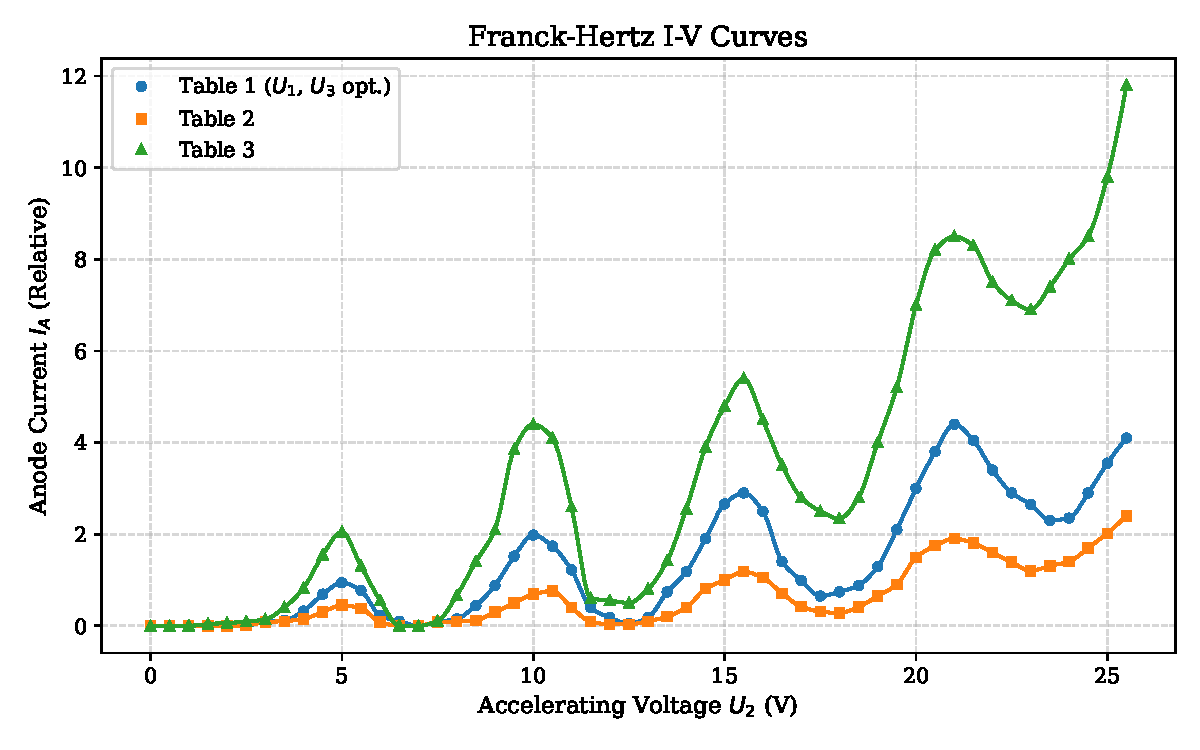
\includegraphics[width=1\textwidth]{franck_hertz_plot.pdf}
    \caption{Franck-Hertz $I-V$ characteristic curves for three different $U_1$ configurations. The periodic maxima and minima are clearly visible superimposed on an increasing background space-charge current.}
    \label{fig:main_plot}
\end{figure}

For the optimal data (Table 1), the positions of the peaks and valleys are extracted:
\begin{itemize}
    \item \textbf{Peaks ($V_p$):} $5.0\text{ V}, 10.0\text{ V}, 15.5\text{ V}, 21.0\text{ V}$
    \item \textbf{Valleys ($V_v$):} $7.0\text{ V}, 12.5\text{ V}, 17.5\text{ V}, 23.5\text{ V}$
\end{itemize}

\subsection{OLS Linear Regression for Excitation Energy ($E_{\text{exc}}$)}
To rigorously determine $E_{\text{exc}}$ and its standard error, we perform an Ordinary Least Squares (OLS) regression of the peak and valley voltages against their index $n$ (where $V_n = m \cdot n + c$). The slope $m$ represents $E_{\text{exc}}$, and the intercept $c$ relates to the contact potential.

\begin{figure}[H]
    \centering
    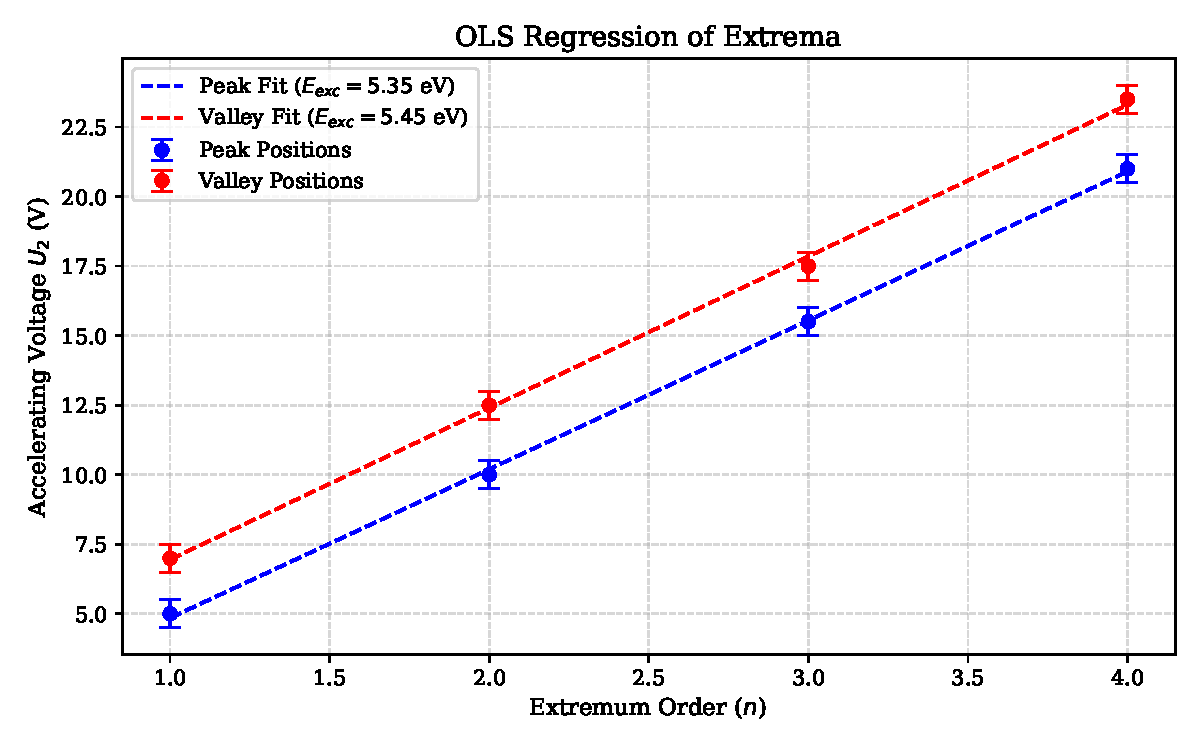
\includegraphics[width=0.75\textwidth]{regression_plot.pdf}
    \caption{OLS linear regression of the peak and valley positions vs. their order $n$, including standard error bands.}
    \label{fig:regression}
\end{figure}
The linear fits yield the following parameters:
\begin{itemize}
    \item \textbf{Peak Regression:} $m_p = 5.350 \pm 0.087\text{ V}$, $R^2 = 0.9995$
    \item \textbf{Valley Regression:} $m_v = 5.450 \pm 0.132\text{ V}$, $R^2 = 0.9988$
\end{itemize}

Combining the slopes using an unweighted average, the experimental excitation energy and its propagated error ($\delta E = \frac{1}{2}\sqrt{\delta m_p^2 + \delta m_v^2}$) are:
\begin{equation}
    E_{\text{exc}} = 5.40 \pm 0.08\text{ eV}
\end{equation}

The theoretical value is $4.9\text{ eV}$. The relative error is $|5.40 - 4.9|/4.9 \approx 10.2\%$, which is acceptable given the $0.5\text{ V}$ step size in data collection.

\subsection{Calculation of Emitted Wavelength ($\lambda$)}
The wavelength of the photon emitted upon de-excitation is given by $\lambda = \frac{hc}{E_{\text{exc}}}$. 
Using $hc = 1240\text{ eV}\cdot\text{nm}$:
\begin{equation}
    \lambda = \frac{1240}{5.40} = 229.63\text{ nm}
\end{equation}
The propagated uncertainty is:
\begin{equation}
    \delta \lambda = \lambda \frac{\delta E_{\text{exc}}}{E_{\text{exc}}} = 229.63 \times \frac{0.0791}{5.400} = 3.36\text{ nm}
\end{equation}
Thus, the emitted wavelength is $\lambda = 229.6 \pm 3.4\text{ nm}$, which lies in the Ultraviolet (UV) spectrum.

% ------------------- Section 5: Answers to Questions -------------------
\section{Answers to Post-Lab Questions}

\subsection*{Q1: What effect does varying $U_1$ have on the $I-V$ curve with respect to $U_2$? Plot the curves and compare.}
The curves are plotted in Fig.~\ref{fig:main_plot}. The control grid voltage $U_1$ acts as an extraction potential that pulls electrons from the space-charge cloud near the heated cathode. Increasing $U_1$ increases the overall thermionic emission current (the baseline of the curves shifts upward significantly). However, if $U_1$ is too high, the energy distribution of the emitted electrons broadens, which can smear out the peaks and valleys, reducing the resolution of the quantum drops.

\subsection*{Q2: What is the excitation energy of the mercury atom? Calculate it from Table 1 and compare it with the exact value.}
As calculated in Section 4 using OLS regression on the extrema of Table 1, the excitation energy is $E_{\text{exc}} = 5.40 \pm 0.08\text{ eV}$. The exact theoretical value is $4.9\text{ eV}$. The discrepancy (approx. $10.2\%$) primarily stems from the large voltage step increments ($0.5\text{ V}$) used during data acquisition, which limits the precision of identifying the exact local extrema.

\subsection*{Q3: What is the wavelength of the light emitted from the excited mercury atoms, and in which region does it lie?}
The calculated wavelength is $\lambda = 229.6 \pm 3.4\text{ nm}$. The theoretical wavelength corresponding to $4.9\text{ eV}$ is $253.7\text{ nm}$. Both values fall squarely in the \textbf{Ultraviolet (UV-C)} region of the electromagnetic spectrum.

\subsection*{Q4: Can a peak corresponding to second-order excitation be observed at higher voltages?}
In the standard Franck-Hertz setup, second-order excitations (e.g., exciting an electron directly to a higher state or ionizing the atom at $10.4\text{ eV}$) are highly unlikely to produce distinct separate peaks. This is because the scattering cross-section for the first excitation ($4.9\text{ eV}$) is orders of magnitude larger. An electron will almost certainly undergo two separate $4.9\text{ eV}$ inelastic collisions rather than surviving to reach $10.4\text{ eV}$ for a single ionizing collision. Therefore, the higher voltage peaks are simply multiple consecutive first-order excitations.

\subsection*{Q5: Why is the position of the first maximum not at the expected potential ($4.9\text{ V}$)?}
The absolute voltage applied by the power supply ($U_2$) does not perfectly equal the kinetic energy of the electrons in the interaction region. The work functions of the cathode metal and the grid metal are different, establishing a \textbf{Contact Potential} ($V_{\text{contact}}$). The true kinetic energy is $E_k = e(U_2 + V_{\text{contact}})$. Because of this offset, the first peak appears at $5.0\text{ V}$ instead of $4.9\text{ V}$. Measuring the distance between consecutive peaks ($\Delta V$) automatically subtracts this contact potential.

\subsection*{Q6: Why does the curve ride on an ascending line?}
The background of the $I-V$ curve follows the $I \propto U_2^{3/2}$ Child-Langmuir law for space-charge-limited current in a vacuum diode. As the accelerating voltage $U_2$ increases, the longitudinal electric field strengthens, effectively sweeping more electrons out of the space-charge cloud around the cathode and driving them to the anode. The inelastic collision drops are merely superimposed on this continuously rising baseline current.

\subsection*{Q7: What is the significance of $U_3$? Can the experiment be performed without it?}
$U_3$ is the \textbf{retarding potential} (or stopping potential). It acts as a high-pass energy filter. If $U_3 = 0$, all electrons—including those that have lost their kinetic energy to inelastic collisions—would eventually drift to the anode and be collected. The ammeter would register a monotonically increasing current without any drops. By applying a small negative $U_3$, we ensure that only electrons retaining sufficient kinetic energy can overcome the barrier, allowing us to detect the inelastic energy losses as sharp drops in current.

\subsection*{Q8: State the significance of the Franck-Hertz experiment.}
The Franck-Hertz experiment provided the first direct, non-spectroscopic confirmation of the Bohr model of the atom. While early evidence for quantization came from observing photon emission spectra, Franck and Hertz proved that energy transfer through mechanical collisions is also strictly quantized. It demonstrated that atoms can only absorb specific, discrete amounts of energy, fundamentally validating quantum mechanics.

\subsection*{Q9: How does the density of mercury atoms affect the $I-V$ curve?}
The density of mercury atoms is controlled by the oven temperature (vapor pressure). If the density is \textbf{too low}, the mean free path of the electrons becomes comparable to the tube length. Electrons will reach the anode without colliding with mercury atoms, resulting in no peaks. If the density is \textbf{too high}, the mean free path is extremely short, leading to excessive elastic scattering that broadens the electron energy distribution and smears out the inelastic peaks entirely. A temperature of $\sim 170^\circ\text{C}$ provides the optimal collision probability.

\subsection*{Q10: What is the advantage of using mercury? What if helium was used?}
Mercury is advantageous because it is a liquid at room temperature and its vapor pressure can be easily and precisely controlled using a simple oven at $170^\circ\text{C}$. Furthermore, its first excitation energy is relatively low ($4.9\text{ eV}$), meaning multiple peaks can be observed within a safe operating voltage range ($0 - 30\text{ V}$). 
If Helium were used, its first excitation energy is very high ($\sim 19.8\text{ eV}$). Observing multiple peaks would require accelerating voltages near $100\text{ V}$, which dramatically increases the risk of Townsend avalanches, arcing, and complete ionization (gas discharge), making it difficult to maintain controlled conditions.

\subsection*{Q11: Determine the quantum states before and after excitation.}
The ground state electron configuration of the valence shell of Mercury is $6s^2$, which is a filled subshell. The total spin is $S=0$ (singlet state).
\begin{itemize}
    \item \textbf{Before Excitation (Ground State):} The term symbol is $^1S_0$. The quantum numbers for the valence electrons are $n=6, l=0, m_l=0$.
    \item \textbf{After Excitation:} The electron transitions to the $6p$ subshell. The most probable transition (due to selection rules and the $\sim 4.9\text{ eV}$ energy gap) is to the triplet state $^3P_1$. The quantum numbers are $n=6, l=1$, and $m_l \in \{-1, 0, 1\}$.
\end{itemize}

\end{document}
